\section{第三次课后作业}

\begin{tcolorbox}[breakable,colback=blue!5!white,colframe=blue!75!black,
 title= 2024-03-11]
 设 $ \xi $ 和 $ \eta $ 联合分布 $ p(0,0)=\frac{1}{3}, p(0,1)=\frac{1}{3}, p(1,0)=0 $, $ p(1,1)=\frac{1}{3} $, 试求:
 
(1) $ H(\xi), H(\eta) $;

(2) $ H(\xi \mid \eta), H(\eta \mid \xi) $;

(3) $ H(\xi, \eta) $;

(4) $ H(\eta)-H(\eta \mid \xi) $;

(5) $ I(\xi ; \eta) $;

(6) 画出上述各信息之间关系的韦恩图.

\tcblower
\begin{center}
     \begin{tabular}{|c|cc|c|}
\hline\diagbox{$ \eta $}{$ \xi $} & 0 & 1 & $ \sum $ \\
\hline 0 & $ \frac{1}{3} $ & 0 & $ \frac{1}{3} $ \\
\hline 1 & $ \frac{1}{3} $ & $ \frac{1}{3} $ & $ \frac{2}{3} $ \\
\hline$ \sum $ & $ \frac{2}{3} $ & $ \frac{1}{3} $ & 1 \\
\hline
\end{tabular}$\quad\Longrightarrow$
$
\xi \sim\left(\begin{array}{cc}
0 & 1 \\
\frac{2}{3} & \frac{1}{3}
\end{array}\right), \quad \eta \sim\left(\begin{array}{cc}
0 & 1 \\
\frac{1}{3} & \frac{2}{3}
\end{array}\right)
$
\end{center}
(1)
$$
\begin{aligned}
H(\xi)  =\sum_{i=0}^{1} p_{i} \log_2 \frac{1}{p_{i}}=\frac{2}{3} \log_2 \frac{3}{2}+\frac{1}{3} \log_2 3 =\frac{2}{3} \log_ 3-\frac{2}{3} \log_ 2+\frac{1}{3} \log_2 3  =\log_2 3-\frac{2}{3}
\end{aligned}
$$
$$
\begin{aligned}
H(\eta)  =\sum_{i=0}^{1} p_{i} \log_2 \frac{1}{p_{i}}=\frac{1}{3} \log_2 3+\frac{2}{3} \log_2 \frac{3}{2}  =\frac{1}{3} \log_2 3+\frac{2}{3} \log_2 3-\frac{2}{3} \log_2 2 \ =\log_2 3-\frac{2}{3}
\end{aligned}
$$
(3)
$$
\begin{aligned}
H(\xi, \eta) & =\sum_{x \in \mathscr{X}} \sum_{x \in \mathscr{Y}} p(x, y) \log \frac{1}{p(x, y)}  =3 \cdot \frac{1}{3} \log_2 3=\log_2 3
\end{aligned}
$$
(2)
$$
\begin{aligned}
H(\eta \mid \xi) & =H(\xi, \eta)-H(\xi)  =\log_2 3-\left(\log_2 3-\frac{2}{3}\right)=\frac{2}{3} \\
H(\xi \mid \eta) & =H(\xi, \eta)-H(\eta)  =\log_2 3-\left(\log_2 3-\frac{2}{3}\right)=\frac{2}{3}
\end{aligned}
$$
(4)
$$
\begin{aligned}
H(\eta)-H(\eta \mid \xi) 
= & \log_2 3-\frac{2}{3}-\frac{2}{3} =  \log_2 3-\frac{4}{3}
\end{aligned}
$$
(5)
$$
\begin{aligned}
I(\xi ; \eta) & =H(\xi)+H(\eta)-H(\xi, \eta)  =(\log_2 3-\frac{2}{3})+(\log_2 3-\frac{2}{3})-\log_2 3  =\log_2 3-\frac{4}{3}
\end{aligned}
$$
(6)

    \centering
    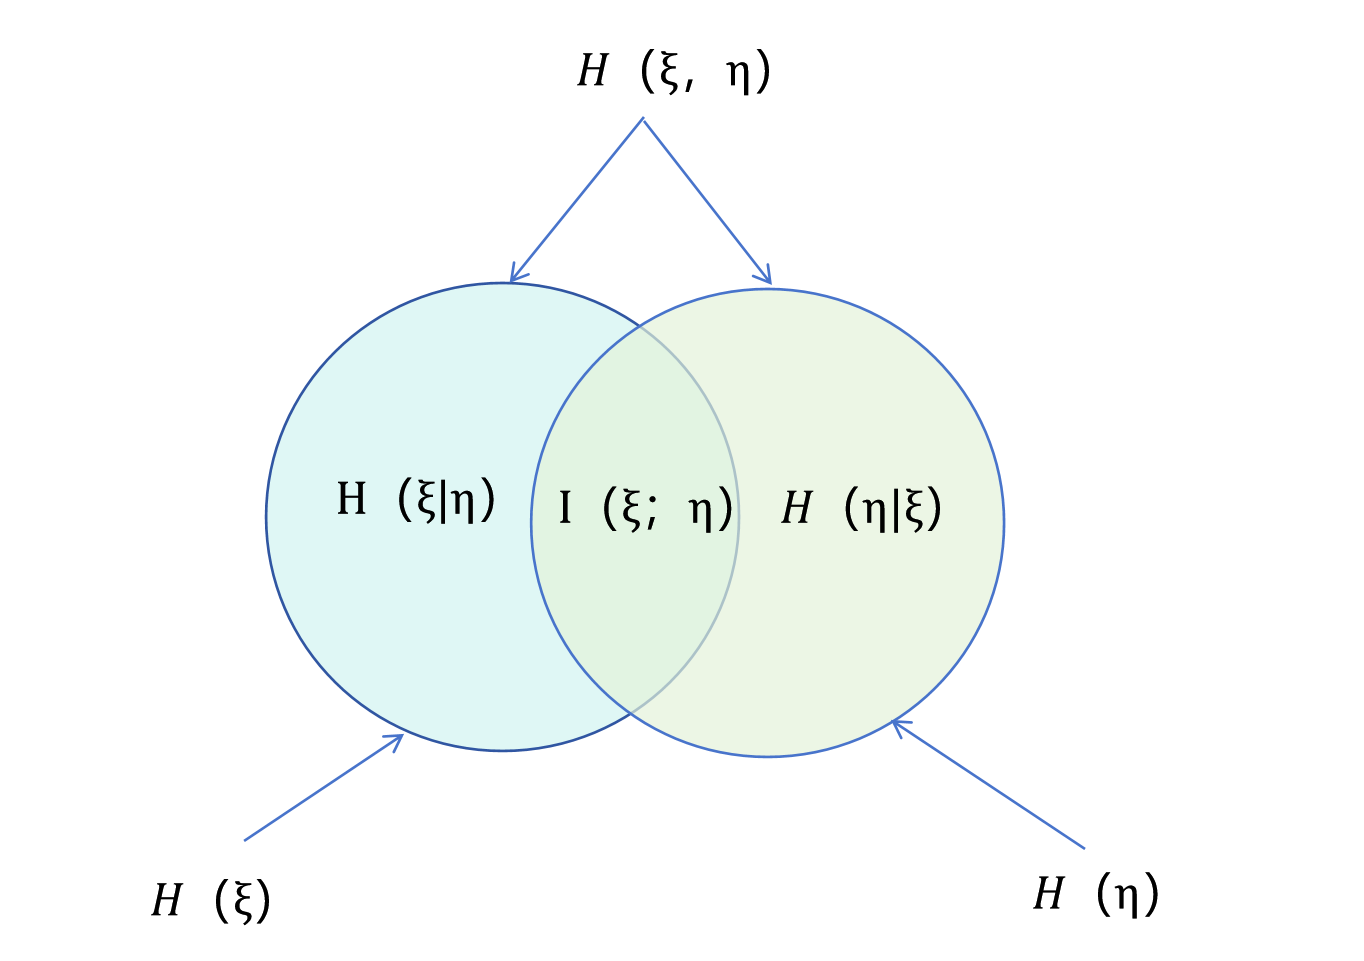
\includegraphics[width=0.4\linewidth]{1.png}
\end{tcolorbox}


\begin{tcolorbox}[breakable,colback=blue!5!white,colframe=blue!75!black,
 title= 2024-03-11]
 设 $ \xi $ 是取 $ m $ 个值 $ x_{1}, x_{2}, \cdots, x_{m} $ 的随机变量, $ p\left(\xi=x_{m}\right)=a $. 证明:
$$
H(\xi)=a \log \frac{1}{a}+(1-a) \log \frac{1}{1-a}+(1-a) H(\eta),
$$
其中 $ \eta $ 是取 $ m-1 $ 个值 $ x_{1},, x_{2}, \cdots, x_{m-1} $ 的随机变量.
$$
p\left(\eta=x_{j}\right) \xlongequal{\text { def }}\frac{p\left(\xi=x_{j}\right)} {(1-a)}, 1 \leqslant j \leqslant m-1 .
$$
进一步, 证
明: $ H(\xi) \leqslant a \log \frac{1}{a}+(1-a) \log \frac{1}{a}+(1-a) \log (m-1) $,并确定其中等号成立的条件.

\tcblower

     证明: 由 $ p\left(\eta=x_{j}\right) \xlongequal{\text { def }}\dfrac{p\left(\xi=x_{j}\right)}{(1-a)}  \Rightarrow p\left(\xi=x_{j}\right)=(1-a) p\left(\eta=x_{j}\right), j=1, \cdots, m-1 . $
$$
\begin{aligned}
\text { 故 } H(\xi)&=a \log \frac{1}{a}+\sum_{j=1}^{m-1} p\left(\xi=x_{j}\right) \log \frac{1}{p\left(\xi=x_{j}\right)} \\
&=a \log \frac{1}{a}+\sum_{j=1}^{m-1}(1-a) p\left(\eta=x_{j}\right) \log \frac{1}{(1-a) p\left(\eta=x_{j}\right)}\\
&=a \log \frac{1}{a}+\sum_{j=1}^{m-1}(1-a) p\left(\eta=x_{j}\right) \log \frac{1}{1-a} +\sum_{j=1}^{m-1}(1-a) p\left(\eta=x_{j}\right) \log \frac{1}{p\left(\eta=x_{j}\right)} \\
&=a \log \frac{1}{a}+(1-a) \log \frac{1}{1-a} \sum_{j=1}^{m-1} p\left(\eta=x_{j}\right) +(1-a) \sum_{j=1}^{m-1} p\left(\eta=x_{j}\right) \log \frac{1}{p\left(\eta=x_{j}\right)} \\
&=a \log \frac{1}{a}+(1-a) \log \frac{1}{1-a}+(1-a) H(\eta)
\end{aligned}
$$

根据熵的最大值定理有 $ H(\eta)\leqslant \log (m-1) $. 因此有
$$ H(\xi) \leqslant a \log \frac{1}{a}+(1-a) \log \frac{1}{a}+(1-a) \log (m-1) $$
等号成立的条件是$ p\left(\eta=x_{j}\right) $ 为等概率分布,
即有
$$
p\left(\eta=x_{j}\right)=\frac{1}{m-1} 
$$
此时$$
 p\left(\xi=x_{j}\right)=\frac{1-a}{m-1}, \quad j=1,2, \cdots, m-1 .
$$

\end{tcolorbox}

